\documentclass[12pt]{article}
\usepackage{graphicx}
\usepackage{epstopdf}
\usepackage[utf8]{inputenc}
\usepackage{url}
\usepackage{color}
\usepackage{amsmath}
\usepackage{amssymb}
\usepackage{booktabs,caption}
\usepackage{caption}
\usepackage{subcaption}
\usepackage[flushleft]{threeparttable}
\usepackage[margin=1in]{geometry}

\DeclareCaptionLabelFormat{blank}{}

\begin{document}
\title{\textbf{ECON 5P04 Research Project: The Effects of Automation on Industry Employment in Canada}}
\author{Zachary Mesic}
\date{\today}
\maketitle

\thispagestyle{empty}
\vfill
\begin{center}
\textbf{BROCK UNIVERSITY}
\break
Master of Business  Economics
\break
Professor Robert W. Dimand
\linebreak
\linebreak
\textbf{\copyright{Zachary Mesic (5820105)}}\\
All rights reserved\\

2020
\end{center}

\newpage

\begin{abstract}
\begin{flushleft}
With the impact technological innovation has had on many aspects of contemporary society, perhaps the most significant has been its effect on the economy. Specfically, how has automation influenced employment across sectors in the economy? This research projects attempts to answer that question by observing the relationship between automation and employment in Canada within recent years. I use a dataset compiled from \textit{Statistics Canada} to track employment levels using the NAICS (North American Industry Classification System) for 8 industry categories. I then use annual survey data collected from two Stats Canada Surveys entitled \textit{Survey of Innovation and Business Strategy (SIBS)} and \textit{Survey of Advanced Technology (SAT)} to track the \% of industries that have adopted `advanced technologies' within recent years, once again using the NAICS industry classficiation. Wages are used in the model as a measure of `skill' that a job possesses. Lastly, I include index variables taken from (Blinder \& Krueger, 2013) in the model to measure the `offshorability' within an industry observe how they too impact employment. I find that over the period \{2009, 2012, 2014, 2017\}, automation does not have a significant impact on the level of employment in a particular industry. Rather, one's wage or `skill' level appears to be a much more likely determinant for employment. I conclude by offering some shortcomings of the model and suggest ways in which future research can be improved upon.
\break
\linebreak
\textbf{Keywords:} automation, employment, industry, Canada, NAICS, occupations.
\end{flushleft}
\end{abstract}

\newpage

\tableofcontents
\listoftables
\listoffigures

\newpage

\section{Background Information}

\begin{flushleft}
Within the literature, the influence of automation on outcomes in the labour market is rather apparent (Frey \& Osbourne, 2013). The fall of employment in ``routine intensive occupations” – i.e. professions that are largely comprised of tasks that follow ``well-defined procedures” that can effortlessly be done by complex algorithms – has been noticed by many authors (Frey \& Osbourne, 2013). Frey and Osbourne (2013) cite studies by Charles, et al. (2013) and Jaimovich and Siu (2012) which stress that currently low rates of employment are mainly due to a continual drop in employment in manufacturing and the vanishing of ``other routine jobs”. Although there is persistent dispute concerning the causes behind the obstinately high rates of unemployment, numerous researchers suggest that ``computer-controlled equipment” is likely a reason for the latest unemployment increases (Brynjolfsson and McAfee, 2011) (Frey \& Osbourne, 2013).
\break
\linebreak
However, some authors have found it difficult to directly observe the effects of automation on labour (Acemoglu \& Restrepo, 2018). Autor, Levy, and Murnane (2003) claim that while there are some outliers, the ``conceptual link” outlining the process in which automation ``complements skilled labor or substitutes for unskilled labor” is not well-established. When it comes to robots specifically, there have been varying results in the research (Acemoglu \& Restrepo, 2018). Some researchers have found that robots do not have an effect on labour (Graetz and Michaels 2015), while others have found that job destruction is caused by the adoption of robots (Acemoglu and Restrepo 2017). Acemoglu and Restrepo (2018) believe that further empirical evidence is necessary to analyze the effects of automation on employment and wages (examined in Acemoglu and Restrepo 2017a). Thus, research that is both systematic empirical in documenting the relationship among AI and labor has been minimally done to this date, and the very few amounts of studies that do exist reach different conclusions (Felton, Raj, \& Seamans, 2018). 
\break
\linebreak
The increased automation of labor-tasks that have led many to believe that labor will become obsolete (Brynjolfsson and McAfee 2014; Akstn 2013; Autor 2015) (Acemoglu \& Restrepo, 2018). In the United States, the most recent drops in the labor share of both ``national income” and the ``employment to population ratio” (e.g., Karabarbounis and Neiman 2014; Oberfield and Raval 2014) have been cited as proof that workforces will find it more and more challenging to battle automation (Acemoglu \& Restrepo, 2018). As digital technologies, robotics, and artificial intelligence enter the economy, a ``relative” or even ``absolute” decrease in compensation will be experienced by workers (Acemoglu \& Restrepo, 2018). 
\break
\linebreak
In a 2017 paper, Acemoglu and Restrepo outline similar concerns. For example, the implementation of robots is associated with lower employment and wages in the labor markets of local communities (Brynjolfsson, Mitchell, \& Rock, 2018). The McKinsey Global Institute conducted a study which found that existing technology can automate approximately half of the tasks completed by workers (Manyika et al. 2017) (Brynjolfsson, Mitchell, \& Rock, 2018). Authors Brynjolfsson and McAfee (2011) insinuate that technological innovation is occurring at an increasing rate, with labour market disruptions becoming more and more apparent due to greater, more complex ``software technologies” deeming human labour obsolete (Frey \& Osbourne, 2013).
\break
\linebreak
Autor (2015) stipulates that although automation can be a substitute for labor, it can also a complement, leading to a rise in output through methods that result in greater labor demand (Autor and Salomons 2017; Bessen 2017) (Acemoglu \& Restrepo, 2018). He argues that over the past two centuries, workers have not been made redundant due to the progress of technology and automation Autor (2015). During the 20th century, there was an increase in the ``employment‐to‐population ratio”; and while there were cyclical fluctuations in the rate of unemployment, a ``long-run increase” is simply not evident (Autor, 2015). Moreover, Felton, Raj, and Seamans (2018) put forth that economic growth can be achieved through the innovation of Artificial Intelligence (AI) (Council of Economic Advisers 2016; Agrawal, Gans, and Goldfarb forthcoming; Brynjolfsson, Rock and Syverson forthcoming). For instance, on average between 1993 and 2007, approximately 0.37 percentage points of yearly GDP growth (making up an estimated one-tenth of GDP growth) for 17 countries was added by higher technology with resemblance to AI called “robotics” (Graetz \& Michaels, 2015) (Felton, Raj, \& Seamans, 2018). 
\break
\linebreak
Authors Mokyr, Vickers, and Ziebarth (2015) share a similar sentiment to Autor (2015). They pose that the severe contemporary worries regarding long-lasting, deep-seated ``technological unemployment”, or a pervasive absence of purpose due to fluctuations in labour trends, appear very improbable to come to fruition. The standard of living will keep improving in many ``dramatic and unexpected ways” due to technological advancements, as has been the case for greater than two centuries. They claim that the central principles of economics will still hold. There will still be an existence of scarcities (time itself in particular). Even in an economy where the abilities of robots and automation have enlarged dramatically, the rule of comparative advantage powerfully implies that the majority of workers will continue to have meaningful tasks to complete (Mokyr, Vickers, \& Ziebarth, 2015).
\break
\linebreak
There appears to be unanimity among certain authors in the field regarding the impact of automation on labor. Where there is fixed capital and exogenous technology in a ``static” form, Acemoglu and Restrepo (2018) document that automation decreases employment and the share of labor and could potentially decrease wages. Whereas, the making of ``new tasks” does the opposite. Kararbounis and Neiman (2013) show that since the early 1980s, within mostly all industries and countries there has been a significant decrease in the labor share globally. They find that the ``elative price” of investment goods has been reduced, and that this is frequently accredited to developments in ``information technology and the computer age” (Kararbounis \& Neiman, 2013). This has incentivized companies to move toward capital and away from labor (Kararbounis \& Neiman, 2013).
\break
\linebreak
Acemoglu \& Restrepo (2019) arrive at similar conclusion, finding over the last three decades, a ``slowdown” in the increase of demand for labor has taken place, with nearly an entire halt throughout the last two. Their methodology involves the study of the development of the ``economy-wide wage bill”, a document that ``combines information on average wages and total employment” and is therefore inciteful regarding fluctuations in total demand for labor (Acemoglu \& Restrepo, 2019). Next, ``industry data” is expended to break down variations in the economy-wide wage bill into “productivity, composition and substitution effects”, and variations in the “task content of production” (Acemoglu \& Restrepo, 2019).
\break
\linebreak
Frey and Osbourne (2013) inspect the anticipated effects of future automation on outcomes in the US market for labor. However, they adopt a different approach, with their main objective being to examine the amount of occupations ``at risk” and the connection amongst a profession's likelihood of automation, pay and education level (Frey \& Osbourne, 2013). Their results suggest that approximately 47 percent of entire employment in the US is in danger (Frey \& Osbourne, 2013). Across a wide range of occupations, current advances in Machine Learning (ML) (a subcategory of AI) will place a significant portion of employment at risk in the immediate future (Frey \& Osbourne, 2013).
\break
\linebreak
There are many authors in the literature who adopt a ``task-based framework” in order to analyze automation’s impact on the demand for labour. For instance, Autor, Levy, and Murnane (2003) show there is a decreasing ``relative industry demand for routine manual and cognitive skills” created by automation and an increasing ``relative demand for non-routine cognitive skills (both interactive and analytical)”. Specifically, they note that in both the variations in ``occupational distributions within detailed industries” and variations in ``skill requirements within detailed occupations”, the demand changes are obvious. Throughout 1970 to 1998, they observe an overall decline in demand for ``routine cognitive and routine manual tasks” and a rise in demand for ``non-routine cognitive tasks” that is focused in sectors that are computer intensive (Autor, Levy, \& Murnane, 2003).
\break
\linebreak
Autor (2015) also uses a task-based approach and has similar findings. He contends that the interaction amongst ``machine and human comparative advantage” is what permits computers to replace employees in accomplishing tasks that are “routine” and ``codifiable”. This is accompanied by an exacerbation in workers’ comparative advantage in providing skills that involve ``problem-solving, adaptability, and creativity”. Acemoglu and Restrepo (2019) define these developments as a ``displacement effect” – the transfer of the task content of production away from labor – and a “reinstatement effect” – new tasks that are created for which a comparative advantage is held by labor (Acemoglu \& Restrepo, 2019). In fact, the task-based framework developed by Acemoglu and Restrepo (2018) suggests that perhaps the greatest influence currently opposing the progression of automation is the construction of new tasks that are intensive in labor – (tasks in which labor possesses a comparative advantage in relation to capital).
\break
\linebreak
However, Acemoglu and Restrepo (2018) note that the surges in per worker output resulting from automation will not result in a proportional growth in labor demand. A “decoupling of wages” and per worker output, accompanied by a decrease in the national income labor share are both consequences of the displacement effect (Acemoglu \& Restrepo, 2018). Traditionally, macroeconomic and labour economic theorists hold that technologies that are productivity-increasing always improve total demand for labor. Yet, the demand for labor, wages and employment can all be negatively impacted by the displacement effect (Acemoglu \& Restrepo, 2018). Thus, these results lie in direct opposition to the widespread beliefs held within the fields of macroeconomics and labor economics (contrary to Mokyr, Vickers, and Ziebarth (2015)) (Acemoglu \& Restrepo, 2018). 
\break
\linebreak
Brynjolfsson, Mitchell and Rock (2018) look at the impact of Machine Learning on tasks as a proxy for the impact of automation of labour demand. They observe the ``suitability of machine learning” (SML) for certain labor activities as a representation of the effect of machine learning on employment (Brynjolfsson, Mitchell, \& Rock, 2018). They highlight three key findings: a) there are at least some tasks that are SML in almost occupations in almost all industries; b) there are little to no professions that possess tasks that are entirely SML; and c) releasing the true potential of ML will necessitate major restructuring of occupations’ content of tasks. Brynjolfsson, Mitchell, and Rock (2018) also highlight that machine learning is a technology unlike previous forms of automation and impacts an extremely distinct ``set of tasks”. Though previous surges of automation were the cause of increased inequality and polarization of wages (Autor and Dorn 2013), they argue that ML will impact highly dissimilar shares of the labour market than former surges (Brynjolfsson, Mitchell, \& Rock, 2018). 
\break
\linebreak
Over the previous few decades, there has been a very prominent trend outlined by many authors in the literature called ``labour market polarization” (Autor, 2015). It is a phenomenon in which the increases in wages disproportionately went to those who occupy the top and bottom ends of the income and skill distributions, leaving out those in the middle (Autor, 2015). Similar conclusions are put forth by Autor and Dorn (2013) who, in addition to the automation of ``routine manufacturing tasks”, measure an underlying labour market shift, with workforces transferring their supply of labour from ``middle-income manufacturing” to ``low-income service” professions (Frey \& Osbourne, 2013). Frey and Osbourne (2013) too forecast a ``truncation” in the contemporary trend towards polarization of the labour market, with automation mainly being restricted to occupations that are low-skill and low-wage. However, they posit that as technology increases, employees who are low-skill will eventually shift towards tasks that are not as exposed to automation – i.e., tasks that require intelligence both creatively and socially.
\break
\linebreak
There appears to be an agreement amongst certain authors regarding how automation’s impact on labour markets should be dealt with in terms of policy. For instance, Autor (2015) argues that distribution will be our primary economic concern, and not scarcity, if automation does indeed deem human labor obsolete. The fundamental arrangement of “income distribution in market economies” is entrenched in “labor scarcity”; throughout their career path, people have (or obtain) a “bundle” of valued “human capital” that, because of its scarce nature, creates a stream of income (Autor, 2015). If automation were to deem human labor unnecessary, we would possess enormous amounts of aggregate wealth, but deciding who possesses it and how to distribute it would prove to be a very difficult task (Autor, 2015). 

\newpage
Similar findings are established by Mokyr, Vickers, and Ziebarth (2015). They hold that there is a definite likelihood that through some form of redistribution of income, the supplementing of workers’ wages for some classes may be necessary. Furthermore, they suggest that the increase in the set of goods provided publicly might also be necessary to encompass specific “primary goods” (Rawls 1971). These may be comprised of “food, housing, education, and health care”, all of which are vital for a life today to thrive (Mokyr, Vickers, \& Ziebarth, 2015).
\break
\linebreak
Perhaps as a caveat to future research, Brynjolfsson, Mitchell, and Rock (2018) stress that a change is necessary in the discussion regarding the consequences of AI on labor. The shift should be towards discussing the “redesign” of occupations and “reengineering of business processes” and should move away from the usual emphasis on complete automation of professions and “pervasive occupational replacement”. Their warnings come from studying the impact of ML technologies on job tasks, which indicate that ML technologies will certainly be extensive, but that the SML of work tasks within jobs widely differs (Brynjolfsson, Mitchell, \& Rock, 2018). It is this “variability” in “task-level SML” that gauges the potential for the restructuring of an occupation, as SML tasks within an occupation that are either high or low may be disconnected and “rebundled” (Brynjolfsson, Mitchell, \& Rock, 2018). Therefore, the primary motivation of scholars, together with managers and businesspersons, should be specifically on the “redesign” of jobs, and not just on automation itself (Brynjolfsson, Mitchell, \& Rock, 2018).
\end{flushleft}

\newpage

\section{Methodology}

\subsection{Employment}

To measure the \% change in employment of industries in Canada, I use a dataset taken from Stats Canada entitled: 
\begin{itemize}
\item Employment by Industry, annual (Survey of Employment, Payrolls and Hours)
\end{itemize}

\begin{figure}[h!]
\centering
\begin{subfigure}{.5\textwidth}
  \centering
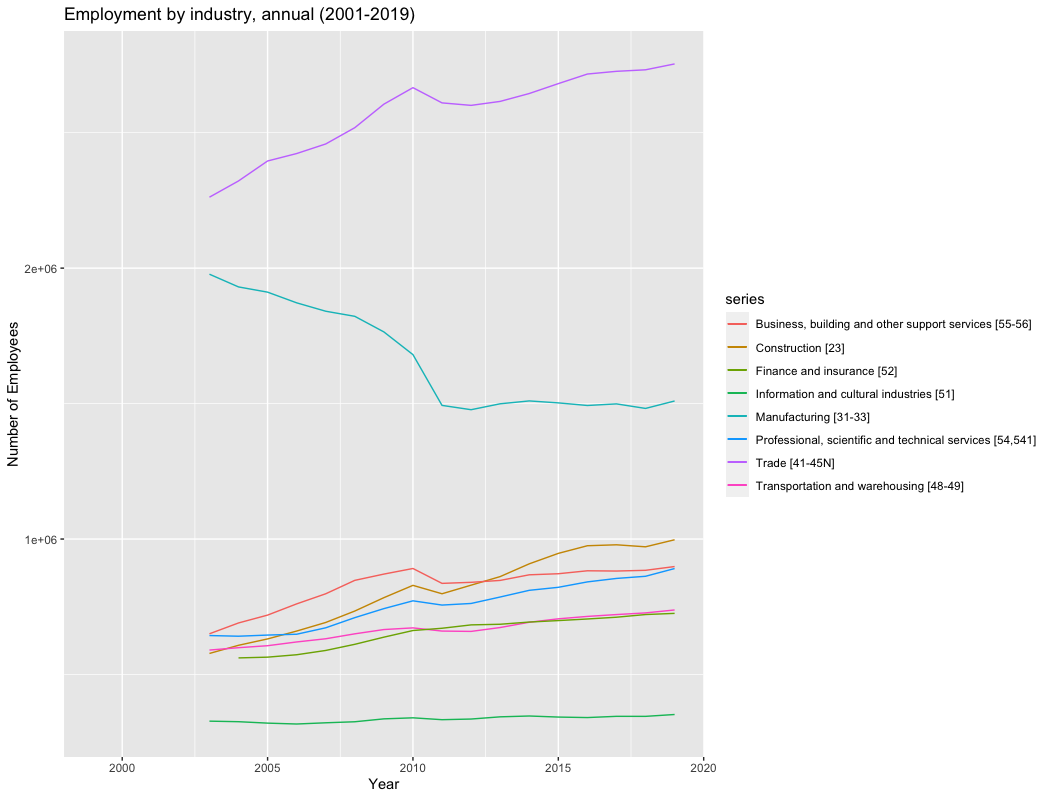
\includegraphics[scale=0.25]{employment.png}
\label{}
\caption{Employment by industry, annual (2001-2019).}
\end{subfigure}%
\begin{subfigure}{.5\textwidth}
  \centering
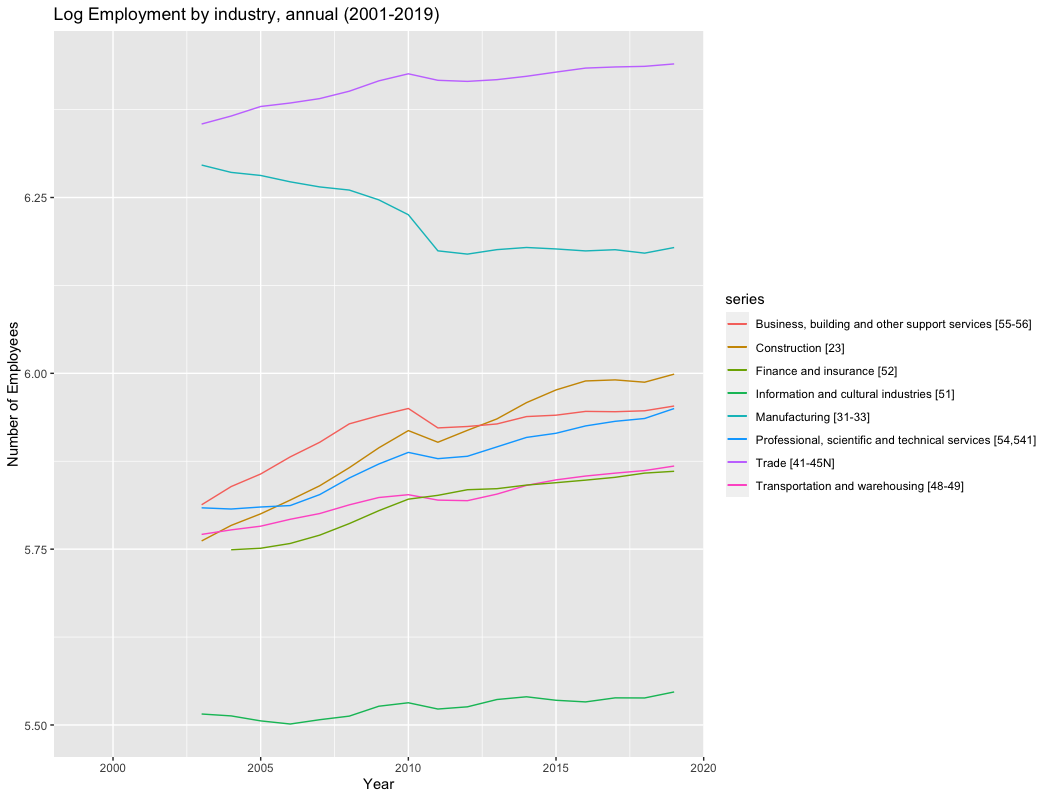
\includegraphics[scale=0.25]{log_employment.png}
\label{}
\caption{Log Employment by industry, annual (2001-2019).}
\end{subfigure}
\captionsetup{textformat=empty,labelformat=blank}
\caption{Employment by industry, annual (2001-2019).}
\caption{Log Employment by industry, annual (2001-2019).}
\end{figure}

I collect aggregate employment levels for the 8 selected NAICS industry classficiations: Construction [23], Manufacturing [31-33], Trade [41-45N], Transportation and warehousing [48-49], Information and cultural industries [51], Finance and insurance [52], Professional, scientific and technical services [54,541], and Business, building and other support services [55-56].
\break
\linebreak
These industry categories were chosen specifically as they are considered 'major' industry categories, in which at least 3\% of the working population occupy (Blinder, \& Krueger, 2013). They were also some of the only categories for which I could find consistent data on with regards to the accompanying variables of the model. 

\newpage

\subsection{Degree of Automation}

To measure the impact of automation on industries, four datasets are taken from two surveys completed by Stats Canada entitled \textit{Survey of Innovation and Business Strategy (SIBS)} and \textit{Survey of Advanced Technology (SAT)} They include:

\begin{itemize}
\item Innovation and business strategy, advanced technology use (2009, 2012) (SIBS)
\item Number of advanced technologies used, by industry and enterprise size (2014) (SAT)
\item Enterprises that use advanced technology, by industry and enterprise size (2014) (SAT)
\item Acquisition or integration of advanced technologies by industry and enterprise size (2014) (SAT)
\item Adoption of advanced business intelligence technologies, by industry and enterprise size (2014) (SAT)
\item Use of advanced or emerging technologies by industry and enterprise size (2017) (SIBS)
\end{itemize}

Each of these surveys captures the degree of automation through dividing the 'type' of automation process being adopted. For example, in Number of advanced technologies used, by industry and enterprise size (2014), they use a "Technology domain" with the following categories: 
\begin{itemize}
\item All domains
\item Advanced material handling, supply chain and logistics technologies
\item Advanced business intelligence technologies
\item Advanced design and information control and advanced processing and fabrication technologies 
\item Advanced green technologies.
\end{itemize}
However, given that each of these surveys, the SIBS and SAT use unique categories or 'domains' to classify automation growth under for each respective dataset, it was impossible to track the automation change directly over these automation categories. Instead, I take a simple average over all of the technological 'domains' for each industry classifications in an effort to aggregate the findings and thus be able to use them for the model. 
\break
\linebreak
The 'degree of automation' variable is a simple average of the percentages of each technology category or 'doman' over each of the datasets listed above.

\newpage

\subsection{Wages}

To measure the \% change in wages of industries in Canada, I use a dataset taken from Stats Canada entitled: 
\begin{itemize}
\item Employee wages by industry, annual (Labour Force Survey)
\end{itemize}

\begin{figure}[h!]
\centering
\begin{subfigure}{.5\textwidth}
  \centering
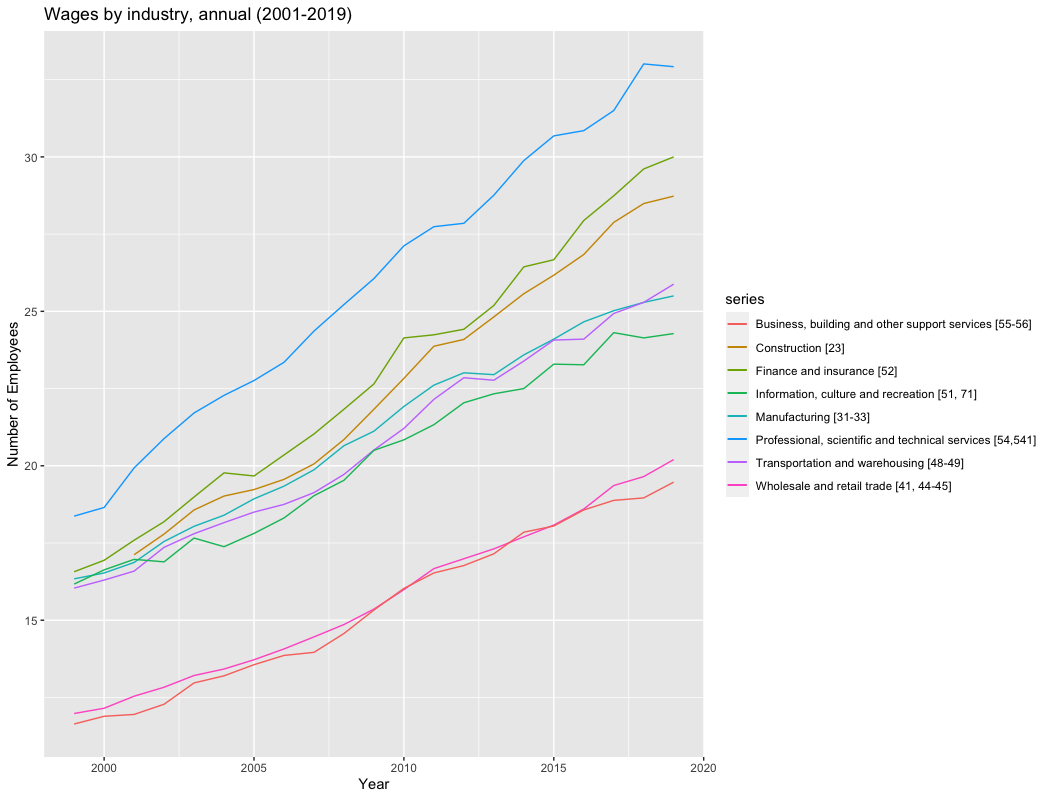
\includegraphics[scale=0.25]{wages.png}
\label{}
\caption{Wages by industry, annual (1999-2019).}
\end{subfigure}%
\begin{subfigure}{.5\textwidth}
  \centering
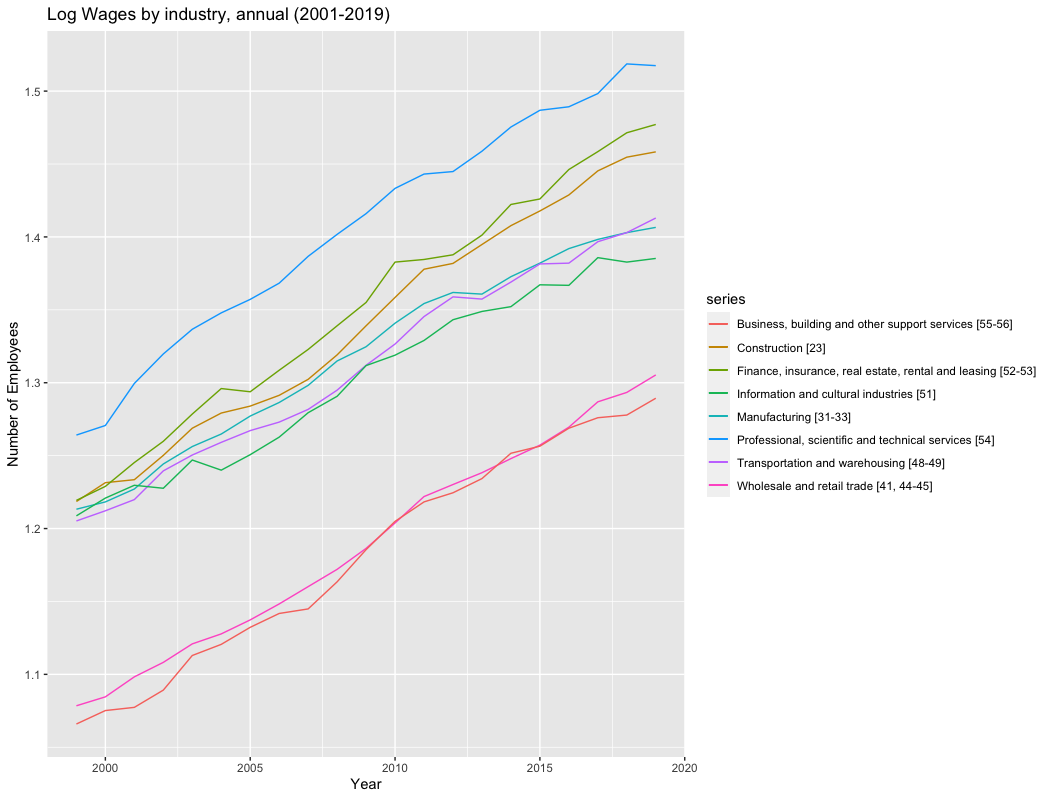
\includegraphics[scale=0.25]{log_wages.png}
\label{}
\caption{Log Wages by industry, annual (1999-2019).}
\end{subfigure}
\captionsetup{textformat=empty,labelformat=blank}
\caption{Wages by industry, annual (1999-2019).}
\caption{Log Wages by industry, annual (1999-2019).}
\end{figure}

\begin{flushleft}
In the model, wages are used to measure the level of ``skill" a particular job within an industry possesses. Since the groupings are at the industry level, wages are then used to measure the overall level of skill within a particular industry.
\break
\linebreak
There are some concerns with using wages as a measure of skill, as outlined by (Green \& Sand, 2013). They argue that if wages represent features other than skill characteristics of workers, (for example, ``wage-setting institutions" or ``compensating differentials"), then can be an issue to measure an occupation's skill level using wages (Green \& Sand, 2013). However, (Goos and Manning, 2007) and (Autor, Katz, and Kearney, 2008) show that high wages in an occupation are correlated with non-routine cognitive tasks and low wages are correlated with non-routine manual tasks. This result suggests that wages is indeed an appropriate proxy for a particular occupation's relative skill level.
\break
\linebreak
This variable can also be thought of as a Rountine-Task Intensity (RTI) as outlined in (Autor \& Dorn, 2013) and (Goos, Manning, and Salomons, 2014). The index is designed to measure the ``routineness of an occupation" (Goos, Manning, and Salomons, 2014). In this model, wages can be thought of as capturing the ``non-routineness" of a job, in the sense that a higher-paying job is less routine and a lower-paying job is more routine.
\end{flushleft}

\newpage

\subsection{Offshorability}

To measure the offshorability of professions in an industry, I rely on figures calculated by (Blinder, \& Krueger, 2013). The following table summarizes their findings:

\begin{table}[!htbp] \centering 
\begin{threeparttable}
  \caption{Offshorability by Industry estimates by (Blinder, \& Krueger, 2013).} 
  \label{} 
\small
\begin{tabular}{@{\extracolsep{5pt}}lccccc} 
 \toprule
\textbf{Offshorability by Industry} \\
\midrule
& & & \textbf{Offshorable (\%)} \\
Industry (NAICS) & All Jobs (\%) & SC & In & Ex \\
\hline \\[-1.8ex] 
Construction (23) & 5.2 & 12.8 & 23.5 & 10.4 \\
Manufacturing (31) &  12 & 27.3	& 32.6 & 50.3 \\
Retail Trade (44) & 10.9 & 17.5 & 20.8	& 10.1 \\
Transport and Warehousing (48) & 3.6 & 11.9 & 22.9 & 9.3 \\
Information (51) & 3.6 & 46.2 & 53.6 & 35.1 \\
Finance and Insurance (52) & 4.7 & 53.2 & 58.2 & 54.8 \\
Professional, Scientific, and Technical & & & & \\
Services (54) & 8.1 & 58.3 & 57.4 & 34.4 \\
Administrative and Support and Waste & & & & \\
Management and Remedial Services (56) & 3.3 & 23 & 20 & 27.8 \\
Educational Services (61) & 9.5 & 15.6 & 14.1 & 6 \\
Health Care and Social Assistance (62) & 13 & 17.4 & 19.8 & 8.5 \\
Arts, Entertainment, and Recreation (71) & 3.2 & 15.3 & 21.9 & 16 \\
Accomodation and Food Services (72) & 6.4 & 9.7 & 3.4 & 0.47 \\
\bottomrule
 \end{tabular}
 \begin{tablenotes}
\item \textit{Note:} NAICS = North American Industry Classification System of the US Census Bureau.
\end{tablenotes}
\end{threeparttable}
\end{table}

\begin{flushleft}
As displayed in the above table, there are three separate measures of the offshorability of an occupation at the industry level: \textbf{Self-Classified method}, \textbf{Inferred method}, and the \textbf{Externally Coded method}. I decide to include all three measures in the model as index variables. Of the three measurements, the Self-Classified method and the Inferred method are ``self-reported" measures (Blinder, \& Krueger, 2013). The Externally Coded method appeaers to be the most precise estimate according to the authors.
\break
\linebreak
\textit{Note:} The resutlts obtained in (Blinder, \& Krueger, 2013) that produce—though not independent—estimates of the fraction of \textbf{US jobs} that are potentially offshorable. Therefore, the model assumes that the degree of offshorability for Canadian occupations is identical to that of American jobs. I  believe this is a fair assumption to make considering the economic and geographic similarities of the two countries.
\end{flushleft}

\newpage

\section{The Model}
The following equation is the regression model used in RStudio to see the impact that the following variables have on employment:
\begingroup
\Large$$logY_i=\beta_0 + \beta_1 log A_i + \beta_2 log w_i  + \beta_3 log x_1  + \beta_4 log x_2 + \beta_5 log x_3 + e_i$$ 
\endgroup
\begin{flushleft}
$Y_i$ - aggregate level of employment in industry $i$
\break
\linebreak
$A_i$ - degree of automation in industry $i$ (measured in \%)
\break
\linebreak
$w_i$ - average hourly wages of employees in indutry $i$, annual (in Canadian dollars)
\break
\linebreak
$x_1$ - degree of offshorability within industry $i$ (Self-Classified method, in \%)
\break
\linebreak
$x_2$ - degree of offshorability within industry $i$ (Inferred method, in \%)
\break
\linebreak
$x_3$ - degree of offshorability within industry $i$ (Externally Coded method, in \%)
\break
\linebreak
$e_i$ - error term
\end{flushleft}

\begin{flushleft}
I offer three variations of the tested model for panel data analysis (Ogwang, 2020). They include the \textbf{Pooling Model}, \textbf{Fixed Effects Model}, and the \textbf{Random Effects Model}. I speak to the advantages and disadvantages of using each model, and compare the individual results they produce.
\break
\begin{enumerate}
\item \textbf{Pooling Model:}
plm(formula = log(df\$Employment) ~ log(df\$Degree\_of\_automation) + 
    log(df\$Wages) + log(df\$OFF\_Self\_Classified) + log(df\$OFF\_Inferred) + 
    log(df\$OFF\_Externally\_Coded), data = df, model = \textbf{"pooling"})
Unbalanced Panel: n = 8, T = 2-4, N = 27
\item \textbf{Fixed Effects Model:}
plm(formula = log(df\$Employment) ~ log(df\$Degree\_of\_automation) + 
    log(df\$Wages) + log(df\$OFF\_Self\_Classified) + log(df\$OFF\_Inferred) + 
    log(df\$OFF\_Externally\_Coded), data = df, model = \textbf{"within"})
Unbalanced Panel: n = 8, T = 2-4, N = 27
\item \textbf{Random Effects Model:}
plm(formula = log(df\$Employment) ~ log(df\$Degree\_of\_automation) + 
    log(df\$Wages) + log(df\$OFF\_Self\_Classified) + log(df\$OFF\_Inferred) + 
    log(df\$OFF\_Externally\_Coded), data = df, model = \textbf{"random"})
Unbalanced Panel: n = 8, T = 2-4, N = 27
\end{enumerate}
\end{flushleft}

\newpage

\section{Results}

\subsection{Pooling Model}

\begin{table}[!htbp] \centering 
\begin{threeparttable}
  \caption{Pooling model regression results.} 
  \label{} 
\begin{tabular}{@{\extracolsep{5pt}}lcccc} 
 \toprule
\midrule
\\
Residuals: \\ 
\hline \\[-1.8ex]
    Min. & 1st Qu. &  Median & 3rd Qu.  &   Max. \\
-1.06293 & -0.26885 & 0.03729 & 0.36963 &  0.71654 \\ 
\\
Coefficients: \\
\hline \\[-1.8ex] 
                  &           Estimate & Std. Error & t-value & Pr($>|t|$)    \\
(Intercept)       &           16.17731 &  1.90344 & 8.4990 & 3.08e-08 *** \\
log(df\$Degree\_of\_automation) & 0.18811 &   0.23710 & 0.7934 & 0.436421    \\
log(df\$Wages)      &       0.51750  &  0.90260 & 0.5733 & 0.572503    \\
log(df\$OFF\_Self\_Classified)  & 1.29594  &  0.60361 & 2.1470 & 0.043627 *  \\
log(df\$OFF\_Inferred)     &    -2.41824 &   0.81597 & -2.9637 & 0.007412 ** \\
log(df\$OFF\_Externally\_Coded) & -0.10969  &  0.25739  & -0.4262 & 0.674327  \\  
\bottomrule
 \end{tabular}
 \begin{tablenotes}
\item \textit{Note:} Signif. codes:  0 ‘***’ 0.001 ‘**’ 0.01 ‘*’ 0.05 ‘.’ 0.1 ‘ ’ 1
\item \
\item Total Sum of Squares:    9.1177
\item Residual Sum of Squares: 5.164
\item R-Squared:      0.43363
\item Adj. R-Squared: 0.29878
\item F-statistic: 3.21565 on 5 and 21 DF, p-value: 0.026054
\end{tablenotes}
  \end{threeparttable}
\end{table} 

The resulting coefficients indicate that the independent variables that are statistically significant are OFF\_Self\_Classified and OFF\_Inferred. We do observe that the coefficient for degree of automation is positive, however statistically insignificant. This indicates that, controlling for all other variables, a one percent increase in technology automation will increase emplyoyment by approximately 18.8 percent. Similarly, a one percent increase in wages will increase employment by approximately 51.75 percent. With the exception of OFF\_Self\_Classified, OFF\_Inferred and OFF\_Externally\_Coded are negatively related with employment. However, the estimated coefficient for the Inferred Method is unusually high, where the Externally Coded method's coefficient is at a much more reasonable level.
\break
\linebreak
The pooled regression model tends to be a poor fit for the data because the data are treated as if there was a single index with no differences among the individual cross section units, ignoring the individual heterogeneity. Therefoure, although the model is appropriate for our index variables for offshoring, we must look to the other models to observe the heterogeneity of employment, wages, and the degree of automation over the given time frame.

\newpage

\subsection{Fixed Effects Model}

\begin{table}[!htbp] \centering 
\begin{threeparttable}
  \caption{Individual fixed effects model regression results.} 
  \label{} 
\begin{tabular}{@{\extracolsep{5pt}}lcccc} 
 \toprule
\midrule
\\
Residuals: \\
\hline \\[-1.8ex]
       Min.  &   1st Qu.  &    Median   &  3rd Qu.   &     Max.  \\
-0.06172735 & -0.01548588  & 0.00072679 &  0.01678546  & 0.04484472  \\
\\
Coefficients: \\
\hline \\[-1.8ex] 
              &                Estimate & Std. Error & t-value  & Pr($>|t|$)     \\
log(df\$Degree\_of\_automation) & -0.011938 &  0.018200 & -0.6559  &  0.5207     \\
log(df\$Wages)      &           0.637480   & 0.110235  & 5.7829 & 2.206e-05 *** \\
\bottomrule
 \end{tabular}
 \begin{tablenotes}
\item \textit{Note:} Signif. codes:  0 ‘***’ 0.001 ‘**’ 0.01 ‘*’ 0.05 ‘.’ 0.1 ‘ ’ 1
\item \
\item Total Sum of Squares:    0.054369
\item Residual Sum of Squares: 0.0153
\item R-Squared:      0.71858
\item Adj. R-Squared: 0.56959
\item F-statistic: 21.7039 on 2 and 17 DF, p-value: 2.087e-05
\end{tablenotes}
  \end{threeparttable}
\end{table} 

\hspace{\parindent}The results indicate that under the fixed effects regression, wages is now a statistically significant variable. Specfically, we see that a one percent increase in wages will lead to an approximate 63.75 increase in emplyoyment. Once again, automation is statistically insignificant. However, this time it is negatigely related to emlpoyment. An increase in the degree of automation by one percent will lead to decrease in emplyoyment by approximately 1.19 percent. 
\break
\linebreak
There exist two main assumptions of the fixed effects regression model. First, the slopes of the regression lines are the same across states and second, the fixed effects captures entirely the time-constant omitted variables. Thus, this is why we do not see the coefficients for offshorability displayed, as they are index variables and are constant. 

\newpage

\subsection{Random Effects Model}

\begin{table}[!htbp] \centering 
\begin{threeparttable}
  \caption{Individual random effects model regression results.} 
  \label{} 
\begin{tabular}{@{\extracolsep{5pt}}lcccc} 
 \toprule
\midrule
\\
Residuals: \\
\hline \\[-1.8ex]
     Min.  &  1st Qu. &    Median  &  3rd Qu.  &     Max.  \\
-0.064050 & -0.020530 &  0.000684 &  0.020715 &  0.044821  \\
 \\
Coefficients: \\
\hline \\[-1.8ex]
             &                 Estimate & Std. Error & z-value &  Pr($>|z|$)     \\
(Intercept)           &        15.122940   & 2.520435  & 6.0001 & 1.972e-09 *** \\
log(df\$Degree\_of\_automation) & -0.011817 &   0.017540 & -0.6738  &   0.5005     \\
log(df\$Wages)         &         0.637305 &   0.106195 &  6.0012 & 1.958e-09 *** \\
log(df\$OFF\_Self\_Classified) &   0.789698  & 1.557193  & 0.5071  &   0.6121     \\
log(df\$OFF\_Inferred)     &     -1.614647 &   1.573987 & -1.0258  &   0.3050     \\
log(df\$OFF\_Externally\_Coded) & -0.114994 &   0.801522 & -0.1435  &   0.8859     \\
\bottomrule
 \end{tabular}
 \begin{tablenotes}
\item \textit{Note:} Signif. codes:  0 ‘***’ 0.001 ‘**’ 0.01 ‘*’ 0.05 ‘.’ 0.1 ‘ ’ 1
\item \ 
\item Total Sum of Squares:    0.072979
\item Residual Sum of Squares: 0.017562
\item R-Squared:      0.76464
\item Adj. R-Squared: 0.70861
\item Chisq: 66.2664 on 5 DF, p-value: 6.1193e-13
\end{tablenotes}
  \end{threeparttable}
\end{table} 

\begin{flushleft}
We see some interesting results arise from the random effects model. First, wages is once again statistically significant and positively related with employment as it was in the pooled and fixed effects model. In the RE model, a one percent increase in wages leads to a 63.7 percent increase in the level of employment. The degree of automation is once again statistically insignificant, where a one percent increase only leads to an approximate 1.01 percent decrease in the level of employment. For offshorability, the resuls are similar to the pooled model. OFF\_Inferred and OFF\_Externally\_Coded are negatively related with employment while OFF\_Self\_Classified is postively related. However, the estimated coefficient for the Inferred Method is unusually high, where the Externally Coded method coefficient is at a much reasonable level.
\break
\linebreak
The random effects model is an alternative to the fixed effects model. In a random effects model, each individual effect is modelled as a random drawing from a probability distribution with mean 0 and constant variance. There are two main components of this model. First, there exists a random intercept term which measures the extent to which an individuals intercept differs from the overall intercept. Second, there is a "traditional" random error term that varies across individuals and time. 

\end{flushleft}

\begin{table}[!htbp] \centering 
  \caption{Oneway (individual) Random Effect Model.} 
  \label{} 
\begin{tabular}{@{\extracolsep{5pt}}lccccc} 
\textbf{Effects:} \\
\hline \\[-1.8ex]
 &  var & std.dev & share & & \\
idiosyncratic & 0.0009  & 0.0300 & 0.001 & &  \\
individual   & 0.6911 &  0.8313 & 0.999 & &  \\
\\
\textbf{theta:} \\
\hline \\[-1.8ex]
   Min. & 1st Qu.  & Median   &  Mean & 3rd Qu. &    Max.  \\
 0.9745 & 0.9792  & 0.9820  & 0.9805 &  0.9820 &  0.9820  \\
\hline \\[-1.8ex]
 \end{tabular}
\end{table} 

An effective way to decide which model is considred the best `fit' for the data is to observe the value of the quasi-within transformation parameter $\theta$. As we can see in the results above, $\theta$ $\approx$ 1. The random effects model lies between the classical pooling model and the fixed effects model which take on values closer to 0 and 1, respectively. Therefore, the estimate is closer to the fixed effects model, since the value is closer to 1.

\subsection{Summary of Findings}

\begin{flushleft}
When it comes to automation and its impact on the aggregate level of employment over the years of \{2009, 2012, 2014, 2017\}, I find no conclusive evidence that automation has a significant impact on employment. In each variation of the model, the estimated coefficient for the degree of automation is statistically insignificant and in the last two (FE and RE), the coefficient is only less than -0.02.
\break
\linebreak
Although the estimated coefficients are a lot higher for offshorability in each case (OFF\_Self\_Classified, OFF\_Inferred, OFF\_Externally\_Coded), there is only one model for which coefficients appears statistically significant and that is in the Pooling Model, where the coefficients themselves are unusually high. This doesn't appear to be substantial enough to conclude a significant impact of offshorability on automation however, given that out of the three, the pooling model is the least reliable. Also, out of the three measures for ohhshoring, the most precise according to Blinder and Krueger (2013) is  OFF\_Externally\_Coded which is not statistically significant. 
\break
\linebreak
The one variable that does prove to be somewhat significant throughout the model is wages. It appears that under the Fixed Effects Model and the Random Effects Model, not only is the estimated coefficient statistically significant, but it is also fairly high, being around 0.637 in both cases. In the case where it is not significant under the Pooling Model, its coefficient is about 0.518. Out of all of the explanatory variables included in the model, we can conclude that wages appears to be the greatest cause for employment. Or, to interpret it differently, a level of one's 'skill' is the greatest cause for employment in a particular industry.
\end{flushleft}

\newpage

\section{Conclusion}

\subsection{Shortcomings of the Model and Potential Solutions}

\begin{flushleft}
In this section, I discuss some of the shortcomings I came across in conducting the research and offer some potential solutions as to how they can be corrected.
\break
\linebreak
Perhaps the most obvious issue that arose from conducting this research was the lack of available data on adoption of advanced technology of firms at the indutry level. The data was only limited to certain years {\{2009, 2012, 2014, 2017\}} thereby making it difficult to observe a linear relationship between variables. Although the gaps in the years of the data could provide important insights into the effects of automation on employment, even though it is also possible that the results would be identical or at least somewhat similar.
\break
\linebreak
Another issue that arises is that the research was strictly conducted at the industry level using the NAICS classification. While it proves informative about automations' effects on overall industries, it does not say much about individual professions across industries and thus does not give a detailed enough analysis of automations' effects on labour demand. I also found limitations in the availability of data on identical industries across datasets, both for technological adoption across the years, and on the offshorability figures provided by (Blinder, \& Krueger, 2013).
\break
\linebreak
A potential solution that I have identified is instead of using industry NAICS classifications to analyze the labour market, it may actually be more informative to use the National Occupational Classification (NOC) developed by Statistics Canada, which delivers a “systematic classification structure“ that organises the complete scope of “occupational activity” for “collecting, analyzing, and disseminating” work-related statistics for information on employment and work-related “program administration” in Canada (NOC, 2020). The NOC codes its occupations based on the skill level and skill type of the job, which thus comes in handy for conveneniently identifying which jobs are high-skill, cognitive versus those that are low-skill and non-cognitive. Using the NOC codes would also eliminate the necessity of having to rely on wages as a measure of a profession's skill, which, as has been previously outlined, can be problematic in it of itself.
\break
\linebreak
Due to the overall lack of availability of data on technological adoption at the industry level, it may be appropriate to search for an entirely different way of modeling the degree to which automation has impacted professions in the labour market. Many researchers have adopted a ``task-based framework" (Autor et al. (2003); Autor (2015))  which aims to identify the shift in the task content of professions (for example, identifying shifts from cognitive, routine to non-cognitive , non-routine tasks). This method would require data and information at the occupational level however, and would require me to move from the industry classification to the occupational level classification. However, given the call from Brynjolfsson, Mitchell, and Rock (2018) to shift the discussion away from the usual emphasis on complete automation of professions  towards the “redesign” of occupations, this may be the appropriate path moving forward.
\end{flushleft}

\newpage

\section{Bibliography}

\begin{flushleft}
\textbf{Papers:}
\begin{itemize}
\item Acemoglu, D. \& Restrepo, P. (2018). Artificial Intelligence, Automation and Work. NBER Working Papers 24196, National Bureau of Economic Research, Inc.
\item Acemoglu, D. \& Restrepo, P. (2019). Automation and New Tasks: How Technology Displaces and Reinstates Labor. Journal of Economic Perspectives, American Economic Association, 33(2), 3-30.
\item Acemoglu, D., \& Restrepo, P. (2018). The Race between Man and Machine: Implications of Technology for Growth, Factor Shares, and Employment. American Economic Review, 108(6): 1488-1542.
\item Autor, D. (2015). Why Are There Still So Many Jobs? The History and Future of Workplace Automation. Journal of Economic Perspectives, 29(3), 3–30.
\item Autor, D., \& Dorn, D. (2013). The Growth of Low-Skill Service Jobs and the Polarization of the US Labor Market. American Economic Review, 103(5), 1553–1597.
\item Autor, D., Levy, F., \& Murnane, R. (2003). “The Skill Content of Recent Technological Change: An Empirical Exploration”, The Quarterly Journal of Economics, 118(4): 1279–1333.
\item Blinder, A., \& Krueger, A. (2013). Alternative Measures of Offshorability: A Survey Approach. Journal of Labor Economics, 31(S1), S97–S128.
\item Brynjolfsson, E., Mitchell, T., \& Rock, D. (2018). What Can Machines Learn, and What Does It Mean for Occupations and the Economy? AEA Papers and Proceedings, 108: 43-47.
\item Felten, E., Raj, M., \& Seamans, R. (2018). A Method to Link Advances in Artificial Intelligence to Occupational Abilities. AEA Papers and Proceedings, 108: 54-57.
\item Frey, C. \& Osborne, M. (2013). The Future of Employment: How Susceptible Are Jobs to Computerisation? Oxford Martin, 114. 10.1016/j.techfore.2016.08.019.
\item Goos, M., Manning, A., \& Salomons, A. (2014). Explaining Job Polarization: Routine-Biased Technological Change and Offshoring. American Economic Review, 104(8), 2509–2526.
\item Green, D., \& Sand, B. (2014). Has the Canadian labour market polarized? Vancouver, British Columbia: Canadian Labour Market and Skills Researcher Network.
\item Karabarbounis, L. \& Neiman, B. (2013). The Global Decline of the Labor Share. NBER Working Papers 19136, National Bureau of Economic Research, Inc.
\item Mokyr, J., Vickers, C., \& Ziebarth, N.L. (2015). The History of Technological Anxiety and the Future of Economic Growth: Is This Time Different? Journal of Economic Perspectives, 29 (3): 31-50.
\item Ogwang, T. (2020). Panel Data Econometrics presented at Brock University in ECON 5P04, St. Catharines.
\end{itemize}

\textbf{Datasets:}
\begin{itemize}
\item NAICS:
\break
https://www150.statcan.gc.ca/n1/en/catalogue/12-501-X (Info)
\item NOC:
https://noc.esdc.gc.ca/Home/AboutTheNoc/5b7072e07630464ba10f0e6f0dcd76e1
\item Employment by Industry, annual (2001-2019):
\break
https://www150.statcan.gc.ca/t1/tbl1/en/cv.action?pid=1410020201\#timeframe 
\item Employee wages by industry, annual (1997-2019):
\break
https://www150.statcan.gc.ca/t1/tbl1/en/tv.action?pid=1410006401
\item Innovation and business strategy, advanced technology use (2009, 2012):
\break
https://www150.statcan.gc.ca/t1/tbl1/en/cv.action?pid=2710013401\#timeframe 
\item Number of advanced technologies used, by industry and enterprise size (2014):
\break
https://www150.statcan.gc.ca/t1/tbl1/en/tv.action?pid=2710027601 
\item Enterprises that use advanced technology, by industry and enterprise size (2014):
\break
https://www150.statcan.gc.ca/t1/tbl1/en/tv.action?pid=2710028801
\item Acquisition or integration of advanced technologies by industry and enterprise size (2014):
\break
https://www150.statcan.gc.ca/t1/tbl1/en/tv.action?pid=2710031101
\item Adoption of advanced business intelligence technologies, by industry and enterprise size (2014):
\break
https://www150.statcan.gc.ca/t1/tbl1/en/tv.action?pid=2710027801 
\item Use of advanced or emerging technologies by industry and enterprise size (2014):
\break
https://www150.statcan.gc.ca/t1/tbl1/en/tv.action?pid=2710036701
\end{itemize}
\end{flushleft}

\newpage

\section{Coding and Output}

\subsection{Coding}

\begin{verbatim}
setwd("~/Documents/NEW MAC/Office/Brock/MBE/ECON 5P04/RESEARCH PROJECT/data")

install.packages("plm")
install.packages("dynlm")
install.packages("psych")
library(dynlm)
library(psych)
library(plm)

df<-read.csv("panel data.csv", header = TRUE)
panel_data<-df
df<-pdata.frame(panel_data)

plm<-plm(log(df$Employment) ~ log(df$Degree_of_automation) + log(df$Wages) + log(df$OFF_Self_Classified) + log(df$OFF_Inferred) + log(df$OFF_Externally_Coded), data = df, model = "pooling")
summary(plm)
plm_within<-plm(log(df$Employment) ~ log(df$Degree_of_automation) + log(df$Wages) + log(df$OFF_Self_Classified) + log(df$OFF_Inferred) + log(df$OFF_Externally_Coded), data = df, model = "within")
summary(plm_within)
plm_random<-plm(log(df$Employment) ~ log(df$Degree_of_automation) + log(df$Wages) + log(df$OFF_Self_Classified) + log(df$OFF_Inferred) + log(df$OFF_Externally_Coded), data = df, model = "random")
summary(plm_random)

setwd("~/Documents/NEW MAC/Office/Brock/MBE/ECON 5P04/RESEARCH PROJECT/data")

install.packages("dynlm")
install.packages("car")
install.packages("psych")
install.packages("ggplot2")
install.packages("forecast")
install.packages("fpp2")
library(dynlm)
library(car)
library(psych)
library("ggplot2")
library("forecast")
library("fpp2")

df<-read.csv("Figures.csv", header = TRUE, check.names=FALSE)

#plot EMPLOYMENT in industries

`Employment in Construction [23]`<-df$`EMP_Construction [23]`
`Employment in Manufacturing [31-33]`<-df$`EMP_Manufacturing [31-33]`
`Employment in Trade [41-45N]`<-df$`EMP_Trade [41-45N]`
`Employment in Transportation and warehousing [48-49]`<-df$`EMP_Transportation and warehousing [48-49]`
`Employment in Information and cultural industries [51]`<-df$`EMP_Information and cultural industries [51]`
`Employment in Finance and insurance [52]`<-df$`EMP_Finance and insurance [52]`
`Employment in Professional, scientific and technical services [54,541]`<-df$`EMP_Professional, scientific and technical services [54,541]`
`Employment in Business, building and other support services [55-56]`<-df$`EMP_Business, building and other support services [55-56]`	

`Employment in Construction [23]`<-ts(`Employment in Construction [23]`,start=c(1999,1), end=c(2019,1))
`Employment in Manufacturing [31-33]`<-ts(`Employment in Manufacturing [31-33]`,start=c(1999,1), end=c(2019,1))
`Employment in Trade [41-45N]`<-ts(`Employment in Trade [41-45N]`,start=c(1999,1), end=c(2019,1))
`Employment in Transportation and warehousing [48-49]`<-ts(`Employment in Transportation and warehousing [48-49]`,start=c(1999,1), end=c(2019,1))
`Employment in Information and cultural industries [51]`<-ts(`Employment in Information and cultural industries [51]`,start=c(1999,1), end=c(2019,1))
`Employment in Finance and insurance [52]`<-ts(`Employment in Finance and insurance [52]`,start=c(1999,1), end=c(2019,1))
`Employment in Professional, scientific and technical services [54,541]`<-ts(`Employment in Professional, scientific and technical services [54,541]`,start=c(1999,1), end=c(2019,1))
`Employment in Business, building and other support services [55-56]`<-ts(`Employment in Business, building and other support services [55-56]`,start=c(1999,1), end=c(2019,1))

`Employment in Construction [23]`<-window(`Employment in Construction [23]`,start=c(1999,1), end=c(2019,1)) 
autoplot(`Employment in Construction [23]`, series = "Construction [23]") + autolayer(`Employment in Manufacturing [31-33]`, series="Manufacturing [31-33]") +
  autolayer(`Employment in Trade [41-45N]`, series="Trade [41-45N]") +
  autolayer(`Employment in Transportation and warehousing [48-49]`, series="Transportation and warehousing [48-49]") +
  autolayer(`Employment in Information and cultural industries [51]`, series="Information and cultural industries [51]") +
  autolayer(`Employment in Finance and insurance [52]`, series="Finance and insurance [52]") +
  autolayer(`Employment in Professional, scientific and technical services [54,541]`, series="Professional, scientific and technical services [54,541]") +
  autolayer(`Employment in Business, building and other support services [55-56]`, series="Business, building and other support services [55-56]") +
  ggtitle("Employment by industry, annual (2001-2019)") + xlab("Year") + ylab("Number of Employees")

#plot log_EMPLOYMENT in industries

`Log Employment in Construction [23]`<-df$`log_EMP_Construction [23]`
`Log Employment in Manufacturing [31-33]`<-df$`log_EMP_Manufacturing [31-33]`
`Log Employment in Trade [41-45N]`<-df$`log_EMP_Trade [41-45N]`
`Log Employment in Transportation and warehousing [48-49]`<-df$`log_EMP_Transportation and warehousing [48-49]`
`Log Employment in Information and cultural industries [51]`<-df$`log_EMP_Information and cultural industries [51]`
`Log Employment in Finance and insurance [52]`<-df$`log_EMP_Finance and insurance [52]`
`Log Employment in Professional, scientific and technical services [54,541]`<-df$`log_EMP_Professional, scientific and technical services [54,541]`
`Log Employment in Business, building and other support services [55-56]`<-df$`log_EMP_Business, building and other support services [55-56]`

`Log Employment in Construction [23]`<-ts(`Log Employment in Construction [23]`,start=c(1999,1), end=c(2019,1))
`Log Employment in Manufacturing [31-33]`<-ts(`Log Employment in Manufacturing [31-33]`,start=c(1999,1), end=c(2019,1))
`Log Employment in Trade [41-45N]`<-ts(`Log Employment in Trade [41-45N]`,start=c(1999,1), end=c(2019,1))
`Log Employment in Transportation and warehousing [48-49]`<-ts(`Log Employment in Transportation and warehousing [48-49]`,start=c(1999,1), end=c(2019,1))
`Log Employment in Information and cultural industries [51]`<-ts(`Log Employment in Information and cultural industries [51]`,start=c(1999,1), end=c(2019,1))
`Log Employment in Finance and insurance [52]`<-ts(`Log Employment in Finance and insurance [52]`,start=c(1999,1), end=c(2019,1))
`Log Employment in Professional, scientific and technical services [54,541]`<-ts(`Log Employment in Professional, scientific and technical services [54,541]`,start=c(1999,1), end=c(2019,1))
`Log Employment in Business, building and other support services [55-56]`<-ts(`Log Employment in Business, building and other support services [55-56]`,start=c(1999,1), end=c(2019,1))

`Log Employment in Construction [23]`<-window(`Log Employment in Construction [23]`,start=c(1999,1), end=c(2019,1)) 
autoplot(`Log Employment in Construction [23]`, series = "Construction [23]") + autolayer(`Log Employment in Manufacturing [31-33]`, series="Manufacturing [31-33]") +
  autolayer(`Log Employment in Trade [41-45N]`, series="Trade [41-45N]") +
  autolayer(`Log Employment in Transportation and warehousing [48-49]`, series="Transportation and warehousing [48-49]") +
  autolayer(`Log Employment in Information and cultural industries [51]`, series="Information and cultural industries [51]") +
  autolayer(`Log Employment in Finance and insurance [52]`, series="Finance and insurance [52]") +
  autolayer(`Log Employment in Professional, scientific and technical services [54,541]`, series="Professional, scientific and technical services [54,541]") +
  autolayer(`Log Employment in Business, building and other support services [55-56]`, series="Business, building and other support services [55-56]") +
  ggtitle("Log Employment by industry, annual (2001-2019)") + xlab("Year") + ylab("Number of Employees")

#plot WAGES in industries

`Wages in Construction [23]`<-df$`WAGE_Construction [23]`
`Wages in Manufacturing [31-33]`<-df$`WAGE_Manufacturing [31-33]`
`Wages in Wholesale and retail trade [41, 44-45]`<-df$`WAGE_Wholesale and retail trade [41, 44-45]`
`Wages in Transportation and warehousing [48-49]`<-df$`WAGE_Transportation and warehousing [48-49]`
`Wages in Information, culture and recreation [51, 71]`<-df$`WAGE_Information, culture and recreation [51, 71]`	
`Wages in Finance, insurance, real estate, rental and leasing [52-53]`<-df$`WAGE_Finance, insurance, real estate, rental and leasing [52-53]`
`Wages in Professional, scientific and technical services [54]`<-df$`WAGE_Professional, scientific and technical services [54]`
`Wages in Business, building and other support services [55-56]`<-df$`WAGE_Business, building and other support services [55-56]`

`Wages in Construction [23]`<-ts(`Wages in Construction [23]`,start=c(1999,1), end=c(2019,1))
`Wages in Manufacturing [31-33]`<-ts(`Wages in Manufacturing [31-33]`,start=c(1999,1), end=c(2019,1))
`Wages in Wholesale and retail trade [41, 44-45]`<-ts(`Wages in Wholesale and retail trade [41, 44-45]`,start=c(1999,1), end=c(2019,1))
`Wages in Transportation and warehousing [48-49]`<-ts(`Wages in Transportation and warehousing [48-49]`,start=c(1999,1), end=c(2019,1))
`Wages in Information, culture and recreation [51, 71]`<-ts(`Wages in Information, culture and recreation [51, 71]`,start=c(1999,1), end=c(2019,1))
`Wages in Finance, insurance, real estate, rental and leasing [52-53]`<-ts(`Wages in Finance, insurance, real estate, rental and leasing [52-53]`,start=c(1999,1), end=c(2019,1))
`Wages in Professional, scientific and technical services [54]`<-ts(`Wages in Professional, scientific and technical services [54]`,start=c(1999,1), end=c(2019,1))
`Wages in Business, building and other support services [55-56]`<-ts(`Wages in Business, building and other support services [55-56]`,start=c(1999,1), end=c(2019,1))

`Wages in Construction [23]`<-window(`Wages in Construction [23]`,start=c(2001,1), end=c(2019,1)) 
autoplot(`Wages in Construction [23]`, series = "Construction [23]") + autolayer(`Wages in Manufacturing [31-33]`, series="Manufacturing [31-33]") +
  autolayer(`Wages in Wholesale and retail trade [41, 44-45]`, series="Wholesale and retail trade [41, 44-45]") +
  autolayer(`Wages in Transportation and warehousing [48-49]`, series="Transportation and warehousing [48-49]") +
  autolayer(`Wages in Information, culture and recreation [51, 71]`, series="Information, culture and recreation [51, 71]") +
  autolayer(`Wages in Finance, insurance, real estate, rental and leasing [52-53]`, series="Finance and insurance [52]") +
  autolayer(`Wages in Professional, scientific and technical services [54]`, series="Professional, scientific and technical services [54,541]") +
  autolayer(`Wages in Business, building and other support services [55-56]`, series="Business, building and other support services [55-56]") +
  ggtitle("Wages by industry, annual (2001-2019)") + xlab("Year") + ylab("Number of Employees")

#plot log_WAGES in industries

`Log Wages in Construction [23]`<-df$`log_WAGE_Construction [23]`
`Log Wages in Manufacturing [31-33]`<-df$`log_WAGE_Manufacturing [31-33]`
`Log Wages in Wholesale and retail trade [41, 44-45]`<-df$`log_WAGE_Wholesale and retail trade [41, 44-45]`
`Log Wages in Transportation and warehousing [48-49]`<-df$`log_WAGE_Transportation and warehousing [48-49]`
`Log Wages in Information, culture and recreation [51, 71]`<-df$`log_WAGE_Information, culture and recreation [51, 71]`
`Log Wages in Finance, insurance, real estate, rental and leasing [52-53]`<-df$`log_WAGE_Finance, insurance, real estate, rental and leasing [52-53]`
`Log Wages in Professional, scientific and technical services [54]`<-df$`log_WAGE_Professional, scientific and technical services [54]`
`Log Wages in Business, building and other support services [55-56]`<-df$`log_WAGE_Business, building and other support services [55-56]`

`Log Wages in Construction [23]`<-ts(`Log Wages in Construction [23]`,start=c(1999,1), end=c(2019,1))
`Log Wages in Manufacturing [31-33]`<-ts(`Log Wages in Manufacturing [31-33]`,start=c(1999,1), end=c(2019,1))
`Log Wages in Wholesale and retail trade [41, 44-45]`<-ts(`Log Wages in Wholesale and retail trade [41, 44-45]`,start=c(1999,1), end=c(2019,1))
`Log Wages in Transportation and warehousing [48-49]`<-ts(`Log Wages in Transportation and warehousing [48-49]`,start=c(1999,1), end=c(2019,1))
`Log Wages in Information, culture and recreation [51, 71]`<-ts(`Log Wages in Information, culture and recreation [51, 71]`,start=c(1999,1), end=c(2019,1))
`Log Wages in Finance, insurance, real estate, rental and leasing [52-53]`<-ts(`Log Wages in Finance, insurance, real estate, rental and leasing [52-53]`,start=c(1999,1), end=c(2019,1))
`Log Wages in Professional, scientific and technical services [54]`<-ts(`Log Wages in Professional, scientific and technical services [54]`,start=c(1999,1), end=c(2019,1))
`Log Wages in Business, building and other support services [55-56]`<-ts(`Log Wages in Business, building and other support services [55-56]`,start=c(1999,1), end=c(2019,1))

`Log Employment in Construction [23]`<-window(`Log Employment in Construction [23]`,start=c(2001,1), end=c(2019,1)) 
autoplot(`Log Wages in Construction [23]`, series = "Construction [23]") + autolayer(`Log Wages in Manufacturing [31-33]`, series="Manufacturing [31-33]") +
  autolayer(`Log Wages in Wholesale and retail trade [41, 44-45]`, series="Wholesale and retail trade [41, 44-45]") +
  autolayer(`Log Wages in Transportation and warehousing [48-49]`, series="Transportation and warehousing [48-49]") +
  autolayer(`Log Wages in Information, culture and recreation [51, 71]`, series="Information and cultural industries [51]") +
  autolayer(`Log Wages in Finance, insurance, real estate, rental and leasing [52-53]`, series="Finance, insurance, real estate, rental and leasing [52-53]") +
  autolayer(`Log Wages in Professional, scientific and technical services [54]`, series="Professional, scientific and technical services [54]") +
  autolayer(`Log Wages in Business, building and other support services [55-56]`, series="Business, building and other support services [55-56]") +
  ggtitle("Log Wages by industry, annual (2001-2019)") + xlab("Year") + ylab("Number of Employees")

\end{verbatim}

\newpage

\subsection{Output}

\begin{verbatim}
R version 3.6.1 (2019-07-05) -- "Action of the Toes"
Copyright (C) 2019 The R Foundation for Statistical Computing
Platform: x86_64-apple-darwin15.6.0 (64-bit)

R is free software and comes with ABSOLUTELY NO WARRANTY.
You are welcome to redistribute it under certain conditions.
Type 'license()' or 'licence()' for distribution details.

  Natural language support but running in an English locale

R is a collaborative project with many contributors.
Type 'contributors()' for more information and
'citation()' on how to cite R or R packages in publications.

Type 'demo()' for some demos, 'help()' for on-line help, or
'help.start()' for an HTML browser interface to help.
Type 'q()' to quit R.

[Workspace loaded from ~/.RData]

> setwd("~/Documents/NEW MAC/Office/Brock/MBE/ECON 5P04/RESEARCH PROJECT/data")
> install.packages("plm")
trying URL 'https://cran.rstudio.com/bin/macosx/el-capitan/contrib/3.6/plm_2.2-3.tgz'
Content type 'application/x-gzip' length 1669369 bytes (1.6 MB)
==================================================
downloaded 1.6 MB


The downloaded binary packages are in
	/var/folders/_q/6113pqk54tx8nbx6c22jwdr40000gn/T//RtmpMDxTEt/downloaded_packages
> install.packages("dynlm")
trying URL 'https://cran.rstudio.com/bin/macosx/el-capitan/contrib/3.6/dynlm_0.3-6.tgz'
Content type 'application/x-gzip' length 53133 bytes (51 KB)
==================================================
downloaded 51 KB


The downloaded binary packages are in
	/var/folders/_q/6113pqk54tx8nbx6c22jwdr40000gn/T//RtmpMDxTEt/downloaded_packages
> install.packages("psych")
trying URL 'https://cran.rstudio.com/bin/macosx/el-capitan/contrib/3.6/psych_1.9.12.31.tgz'
Content type 'application/x-gzip' length 3801830 bytes (3.6 MB)
==================================================
downloaded 3.6 MB


The downloaded binary packages are in
	/var/folders/_q/6113pqk54tx8nbx6c22jwdr40000gn/T//RtmpMDxTEt/downloaded_packages
> library(dynlm)
Loading required package: zoo

Attaching package: ‘zoo’

The following objects are masked from ‘package:base’:

    as.Date, as.Date.numeric

> library(psych)
> library(plm)
> df<-read.csv("panel data.csv", header = TRUE)
> panel_data<-df
> df<-pdata.frame(panel_data)
> plm<-plm(log(df$Employment) ~ log(df$Degree_of_automation) + log(df$Wages) + log(df$OFF_Self_Classified) + log(df$OFF_Inferred) + log(df$OFF_Externally_Coded), data = df, model = "pooling")
> summary(plm)
Pooling Model

Call:
plm(formula = log(df$Employment) ~ log(df$Degree_of_automation) + 
    log(df$Wages) + log(df$OFF_Self_Classified) + log(df$OFF_Inferred) + 
    log(df$OFF_Externally_Coded), data = df, model = "pooling")

Unbalanced Panel: n = 8, T = 2-4, N = 27

Residuals:
    Min.  1st Qu.   Median  3rd Qu.     Max. 
-1.06293 -0.26885  0.03729  0.36963  0.71654 

Coefficients:
                             Estimate Std. Error t-value Pr(>|t|)    
(Intercept)                  16.17731    1.90344  8.4990 3.08e-08 ***
log(df$Degree_of_automation)  0.18811    0.23710  0.7934 0.436421    
log(df$Wages)                 0.51750    0.90260  0.5733 0.572503    
log(df$OFF_Self_Classified)   1.29594    0.60361  2.1470 0.043627 *  
log(df$OFF_Inferred)         -2.41824    0.81597 -2.9637 0.007412 ** 
log(df$OFF_Externally_Coded) -0.10969    0.25739 -0.4262 0.674327    
---
Signif. codes:  0 ‘***’ 0.001 ‘**’ 0.01 ‘*’ 0.05 ‘.’ 0.1 ‘ ’ 1

Total Sum of Squares:    9.1177
Residual Sum of Squares: 5.164
R-Squared:      0.43363
Adj. R-Squared: 0.29878
F-statistic: 3.21565 on 5 and 21 DF, p-value: 0.026054
> plm_within<-plm(log(df$Employment) ~ log(df$Degree_of_automation) + log(df$Wages) + log(df$OFF_Self_Classified) + log(df$OFF_Inferred) + log(df$OFF_Externally_Coded), data = df, model = "within")
> summary(plm_within)
Oneway (individual) effect Within Model

Call:
plm(formula = log(df$Employment) ~ log(df$Degree_of_automation) + 
    log(df$Wages) + log(df$OFF_Self_Classified) + log(df$OFF_Inferred) + 
    log(df$OFF_Externally_Coded), data = df, model = "within")

Unbalanced Panel: n = 8, T = 2-4, N = 27

Residuals:
       Min.     1st Qu.      Median     3rd Qu.        Max. 
-0.06172735 -0.01548588  0.00072679  0.01678546  0.04484472 

Coefficients:
                              Estimate Std. Error t-value  Pr(>|t|)    
log(df$Degree_of_automation) -0.011938   0.018200 -0.6559    0.5207    
log(df$Wages)                 0.637480   0.110235  5.7829 2.206e-05 ***
---
Signif. codes:  0 ‘***’ 0.001 ‘**’ 0.01 ‘*’ 0.05 ‘.’ 0.1 ‘ ’ 1

Total Sum of Squares:    0.054369
Residual Sum of Squares: 0.0153
R-Squared:      0.71858
Adj. R-Squared: 0.56959
F-statistic: 21.7039 on 2 and 17 DF, p-value: 2.087e-05
> plm_random<-plm(log(df$Employment) ~ log(df$Degree_of_automation) + log(df$Wages) + log(df$OFF_Self_Classified) + log(df$OFF_Inferred) + log(df$OFF_Externally_Coded), data = df, model = "random")
> summary(plm_random)
Oneway (individual) effect Random Effect Model 
   (Swamy-Arora's transformation)

Call:
plm(formula = log(df$Employment) ~ log(df$Degree_of_automation) + 
    log(df$Wages) + log(df$OFF_Self_Classified) + log(df$OFF_Inferred) + 
    log(df$OFF_Externally_Coded), data = df, model = "random")

Unbalanced Panel: n = 8, T = 2-4, N = 27

Effects:
                 var std.dev share
idiosyncratic 0.0009  0.0300 0.001
individual    0.6911  0.8313 0.999
theta:
   Min. 1st Qu.  Median    Mean 3rd Qu.    Max. 
 0.9745  0.9792  0.9820  0.9805  0.9820  0.9820 

Residuals:
     Min.   1st Qu.    Median      Mean   3rd Qu.      Max. 
-0.064050 -0.020530 -0.005126  0.000684  0.020715  0.044821 

Coefficients:
                              Estimate Std. Error z-value  Pr(>|z|)    
(Intercept)                  15.122940   2.520435  6.0001 1.972e-09 ***
log(df$Degree_of_automation) -0.011817   0.017540 -0.6738    0.5005    
log(df$Wages)                 0.637305   0.106195  6.0012 1.958e-09 ***
log(df$OFF_Self_Classified)   0.789698   1.557193  0.5071    0.6121    
log(df$OFF_Inferred)         -1.614647   1.573987 -1.0258    0.3050    
log(df$OFF_Externally_Coded) -0.114994   0.801522 -0.1435    0.8859    
---
Signif. codes:  0 ‘***’ 0.001 ‘**’ 0.01 ‘*’ 0.05 ‘.’ 0.1 ‘ ’ 1

Total Sum of Squares:    0.072979
Residual Sum of Squares: 0.017562
R-Squared:      0.76464
Adj. R-Squared: 0.70861
Chisq: 66.2664 on 5 DF, p-value: 6.1193e-13

setwd("~/Documents/NEW MAC/Office/Brock/MBE/ECON 5P04/RESEARCH PROJECT/data")

install.packages("dynlm")
install.packages("car")
install.packages("psych")
install.packages("ggplot2")
install.packages("forecast")
install.packages("fpp2")
library(dynlm)
library(car)
library(psych)
library("ggplot2")
library("forecast")
library("fpp2")

df<-read.csv("Figures.csv", header = TRUE, check.names=FALSE)

#plot EMPLOYMENT in industries

`Employment in Construction [23]`<-df$`EMP_Construction [23]`
`Employment in Manufacturing [31-33]`<-df$`EMP_Manufacturing [31-33]`
`Employment in Trade [41-45N]`<-df$`EMP_Trade [41-45N]`
`Employment in Transportation and warehousing [48-49]`<-df$`EMP_Transportation and warehousing [48-49]`
`Employment in Information and cultural industries [51]`<-df$`EMP_Information and cultural industries [51]`
`Employment in Finance and insurance [52]`<-df$`EMP_Finance and insurance [52]`
`Employment in Professional, scientific and technical services [54,541]`<-df$`EMP_Professional, scientific and technical services [54,541]`
`Employment in Business, building and other support services [55-56]`<-df$`EMP_Business, building and other support services [55-56]`	

`Employment in Construction [23]`<-ts(`Employment in Construction [23]`,start=c(1999,1), end=c(2019,1))
`Employment in Manufacturing [31-33]`<-ts(`Employment in Manufacturing [31-33]`,start=c(1999,1), end=c(2019,1))
`Employment in Trade [41-45N]`<-ts(`Employment in Trade [41-45N]`,start=c(1999,1), end=c(2019,1))
`Employment in Transportation and warehousing [48-49]`<-ts(`Employment in Transportation and warehousing [48-49]`,start=c(1999,1), end=c(2019,1))
`Employment in Information and cultural industries [51]`<-ts(`Employment in Information and cultural industries [51]`,start=c(1999,1), end=c(2019,1))
`Employment in Finance and insurance [52]`<-ts(`Employment in Finance and insurance [52]`,start=c(1999,1), end=c(2019,1))
`Employment in Professional, scientific and technical services [54,541]`<-ts(`Employment in Professional, scientific and technical services [54,541]`,start=c(1999,1), end=c(2019,1))
`Employment in Business, building and other support services [55-56]`<-ts(`Employment in Business, building and other support services [55-56]`,start=c(1999,1), end=c(2019,1))

`Employment in Construction [23]`<-window(`Employment in Construction [23]`,start=c(1999,1), end=c(2019,1)) 
autoplot(`Employment in Construction [23]`, series = "Construction [23]") + autolayer(`Employment in Manufacturing [31-33]`, series="Manufacturing [31-33]") +
  autolayer(`Employment in Trade [41-45N]`, series="Trade [41-45N]") +
  autolayer(`Employment in Transportation and warehousing [48-49]`, series="Transportation and warehousing [48-49]") +
  autolayer(`Employment in Information and cultural industries [51]`, series="Information and cultural industries [51]") +
  autolayer(`Employment in Finance and insurance [52]`, series="Finance and insurance [52]") +
  autolayer(`Employment in Professional, scientific and technical services [54,541]`, series="Professional, scientific and technical services [54,541]") +
  autolayer(`Employment in Business, building and other support services [55-56]`, series="Business, building and other support services [55-56]") +
  ggtitle("Employment by industry, annual (2001-2019)") + xlab("Year") + ylab("Number of Employees")

#plot log_EMPLOYMENT in industries

`Log Employment in Construction [23]`<-df$`log_EMP_Construction [23]`
`Log Employment in Manufacturing [31-33]`<-df$`log_EMP_Manufacturing [31-33]`
`Log Employment in Trade [41-45N]`<-df$`log_EMP_Trade [41-45N]`
`Log Employment in Transportation and warehousing [48-49]`<-df$`log_EMP_Transportation and warehousing [48-49]`
`Log Employment in Information and cultural industries [51]`<-df$`log_EMP_Information and cultural industries [51]`
`Log Employment in Finance and insurance [52]`<-df$`log_EMP_Finance and insurance [52]`
`Log Employment in Professional, scientific and technical services [54,541]`<-df$`log_EMP_Professional, scientific and technical services [54,541]`
`Log Employment in Business, building and other support services [55-56]`<-df$`log_EMP_Business, building and other support services [55-56]`

`Log Employment in Construction [23]`<-ts(`Log Employment in Construction [23]`,start=c(1999,1), end=c(2019,1))
`Log Employment in Manufacturing [31-33]`<-ts(`Log Employment in Manufacturing [31-33]`,start=c(1999,1), end=c(2019,1))
`Log Employment in Trade [41-45N]`<-ts(`Log Employment in Trade [41-45N]`,start=c(1999,1), end=c(2019,1))
`Log Employment in Transportation and warehousing [48-49]`<-ts(`Log Employment in Transportation and warehousing [48-49]`,start=c(1999,1), end=c(2019,1))
`Log Employment in Information and cultural industries [51]`<-ts(`Log Employment in Information and cultural industries [51]`,start=c(1999,1), end=c(2019,1))
`Log Employment in Finance and insurance [52]`<-ts(`Log Employment in Finance and insurance [52]`,start=c(1999,1), end=c(2019,1))
`Log Employment in Professional, scientific and technical services [54,541]`<-ts(`Log Employment in Professional, scientific and technical services [54,541]`,start=c(1999,1), end=c(2019,1))
`Log Employment in Business, building and other support services [55-56]`<-ts(`Log Employment in Business, building and other support services [55-56]`,start=c(1999,1), end=c(2019,1))

`Log Employment in Construction [23]`<-window(`Log Employment in Construction [23]`,start=c(1999,1), end=c(2019,1)) 
autoplot(`Log Employment in Construction [23]`, series = "Construction [23]") + autolayer(`Log Employment in Manufacturing [31-33]`, series="Manufacturing [31-33]") +
  autolayer(`Log Employment in Trade [41-45N]`, series="Trade [41-45N]") +
  autolayer(`Log Employment in Transportation and warehousing [48-49]`, series="Transportation and warehousing [48-49]") +
  autolayer(`Log Employment in Information and cultural industries [51]`, series="Information and cultural industries [51]") +
  autolayer(`Log Employment in Finance and insurance [52]`, series="Finance and insurance [52]") +
  autolayer(`Log Employment in Professional, scientific and technical services [54,541]`, series="Professional, scientific and technical services [54,541]") +
  autolayer(`Log Employment in Business, building and other support services [55-56]`, series="Business, building and other support services [55-56]") +
  ggtitle("Log Employment by industry, annual (2001-2019)") + xlab("Year") + ylab("Number of Employees")

#plot WAGES in industries

`Wages in Construction [23]`<-df$`WAGE_Construction [23]`
`Wages in Manufacturing [31-33]`<-df$`WAGE_Manufacturing [31-33]`
`Wages in Wholesale and retail trade [41, 44-45]`<-df$`WAGE_Wholesale and retail trade [41, 44-45]`
`Wages in Transportation and warehousing [48-49]`<-df$`WAGE_Transportation and warehousing [48-49]`
`Wages in Information, culture and recreation [51, 71]`<-df$`WAGE_Information, culture and recreation [51, 71]`	
`Wages in Finance, insurance, real estate, rental and leasing [52-53]`<-df$`WAGE_Finance, insurance, real estate, rental and leasing [52-53]`
`Wages in Professional, scientific and technical services [54]`<-df$`WAGE_Professional, scientific and technical services [54]`
`Wages in Business, building and other support services [55-56]`<-df$`WAGE_Business, building and other support services [55-56]`

`Wages in Construction [23]`<-ts(`Wages in Construction [23]`,start=c(1999,1), end=c(2019,1))
`Wages in Manufacturing [31-33]`<-ts(`Wages in Manufacturing [31-33]`,start=c(1999,1), end=c(2019,1))
`Wages in Wholesale and retail trade [41, 44-45]`<-ts(`Wages in Wholesale and retail trade [41, 44-45]`,start=c(1999,1), end=c(2019,1))
`Wages in Transportation and warehousing [48-49]`<-ts(`Wages in Transportation and warehousing [48-49]`,start=c(1999,1), end=c(2019,1))
`Wages in Information, culture and recreation [51, 71]`<-ts(`Wages in Information, culture and recreation [51, 71]`,start=c(1999,1), end=c(2019,1))
`Wages in Finance, insurance, real estate, rental and leasing [52-53]`<-ts(`Wages in Finance, insurance, real estate, rental and leasing [52-53]`,start=c(1999,1), end=c(2019,1))
`Wages in Professional, scientific and technical services [54]`<-ts(`Wages in Professional, scientific and technical services [54]`,start=c(1999,1), end=c(2019,1))
`Wages in Business, building and other support services [55-56]`<-ts(`Wages in Business, building and other support services [55-56]`,start=c(1999,1), end=c(2019,1))

`Wages in Construction [23]`<-window(`Wages in Construction [23]`,start=c(2001,1), end=c(2019,1)) 
autoplot(`Wages in Construction [23]`, series = "Construction [23]") + autolayer(`Wages in Manufacturing [31-33]`, series="Manufacturing [31-33]") +
  autolayer(`Wages in Wholesale and retail trade [41, 44-45]`, series="Wholesale and retail trade [41, 44-45]") +
  autolayer(`Wages in Transportation and warehousing [48-49]`, series="Transportation and warehousing [48-49]") +
  autolayer(`Wages in Information, culture and recreation [51, 71]`, series="Information, culture and recreation [51, 71]") +
  autolayer(`Wages in Finance, insurance, real estate, rental and leasing [52-53]`, series="Finance and insurance [52]") +
  autolayer(`Wages in Professional, scientific and technical services [54]`, series="Professional, scientific and technical services [54,541]") +
  autolayer(`Wages in Business, building and other support services [55-56]`, series="Business, building and other support services [55-56]") +
  ggtitle("Wages by industry, annual (2001-2019)") + xlab("Year") + ylab("Number of Employees")

#plot log_WAGES in industries

`Log Wages in Construction [23]`<-df$`log_WAGE_Construction [23]`
`Log Wages in Manufacturing [31-33]`<-df$`log_WAGE_Manufacturing [31-33]`
`Log Wages in Wholesale and retail trade [41, 44-45]`<-df$`log_WAGE_Wholesale and retail trade [41, 44-45]`
`Log Wages in Transportation and warehousing [48-49]`<-df$`log_WAGE_Transportation and warehousing [48-49]`
`Log Wages in Information, culture and recreation [51, 71]`<-df$`log_WAGE_Information, culture and recreation [51, 71]`
`Log Wages in Finance, insurance, real estate, rental and leasing [52-53]`<-df$`log_WAGE_Finance, insurance, real estate, rental and leasing [52-53]`
`Log Wages in Professional, scientific and technical services [54]`<-df$`log_WAGE_Professional, scientific and technical services [54]`
`Log Wages in Business, building and other support services [55-56]`<-df$`log_WAGE_Business, building and other support services [55-56]`

`Log Wages in Construction [23]`<-ts(`Log Wages in Construction [23]`,start=c(1999,1), end=c(2019,1))
`Log Wages in Manufacturing [31-33]`<-ts(`Log Wages in Manufacturing [31-33]`,start=c(1999,1), end=c(2019,1))
`Log Wages in Wholesale and retail trade [41, 44-45]`<-ts(`Log Wages in Wholesale and retail trade [41, 44-45]`,start=c(1999,1), end=c(2019,1))
`Log Wages in Transportation and warehousing [48-49]`<-ts(`Log Wages in Transportation and warehousing [48-49]`,start=c(1999,1), end=c(2019,1))
`Log Wages in Information, culture and recreation [51, 71]`<-ts(`Log Wages in Information, culture and recreation [51, 71]`,start=c(1999,1), end=c(2019,1))
`Log Wages in Finance, insurance, real estate, rental and leasing [52-53]`<-ts(`Log Wages in Finance, insurance, real estate, rental and leasing [52-53]`,start=c(1999,1), end=c(2019,1))
`Log Wages in Professional, scientific and technical services [54]`<-ts(`Log Wages in Professional, scientific and technical services [54]`,start=c(1999,1), end=c(2019,1))
`Log Wages in Business, building and other support services [55-56]`<-ts(`Log Wages in Business, building and other support services [55-56]`,start=c(1999,1), end=c(2019,1))

`Log Employment in Construction [23]`<-window(`Log Employment in Construction [23]`,start=c(2001,1), end=c(2019,1)) 
autoplot(`Log Wages in Construction [23]`, series = "Construction [23]") + autolayer(`Log Wages in Manufacturing [31-33]`, series="Manufacturing [31-33]") +
  autolayer(`Log Wages in Wholesale and retail trade [41, 44-45]`, series="Wholesale and retail trade [41, 44-45]") +
  autolayer(`Log Wages in Transportation and warehousing [48-49]`, series="Transportation and warehousing [48-49]") +
  autolayer(`Log Wages in Information, culture and recreation [51, 71]`, series="Information and cultural industries [51]") +
  autolayer(`Log Wages in Finance, insurance, real estate, rental and leasing [52-53]`, series="Finance, insurance, real estate, rental and leasing [52-53]") +
  autolayer(`Log Wages in Professional, scientific and technical services [54]`, series="Professional, scientific and technical services [54]") +
  autolayer(`Log Wages in Business, building and other support services [55-56]`, series="Business, building and other support services [55-56]") +
  ggtitle("Log Wages by industry, annual (2001-2019)") + xlab("Year") + ylab("Number of Employees")

\end{verbatim}

\end{document}